\documentclass[11pt,a4paper]{article}

\usepackage{iftex}
\ifPDFTeX
  \usepackage[utf8]{inputenc}
  \usepackage[T1]{fontenc}
  \usepackage{lmodern}
\else
  \usepackage{fontspec} % XeLaTeX / LuaLaTeX / Tectonic
\fi
\usepackage[margin=2.2cm]{geometry}
\usepackage{amsmath}
\usepackage{graphicx}
\usepackage{booktabs}
\usepackage{float}
\usepackage{algorithm}
\usepackage{algpseudocode}
\usepackage{xcolor}
\usepackage{xurl}
\usepackage{hyperref}

\hypersetup{colorlinks=true, linkcolor=black, urlcolor=blue!60!black}
\setlength{\parindent}{0pt}
\setlength{\parskip}{6pt}

% a list of node indices, wrapped freely
\newcommand{\nodelist}[1]{\par\nopagebreak{\small\ttfamily\raggedright #1\par}}

\title{Lab 4: The use of candidate moves in local search}
\author{Aleksander Hański, Kacper Kuźnik}
\date{}

\begin{document}
\maketitle

\textbf{Source code:}\\
\url{https://github.com/aleksanderhanski/evolutionary-computation/tree/main/lab4-candidate-moves}

% ---------------------------------------------------------------
\section{Description of the problem}

We are given a set of nodes. Each node has $x$ and $y$ coordinates in a plane and a cost. The goal
is to select exactly 50\% of the nodes (rounded up if the number of nodes is odd) and form a
Hamiltonian cycle through the selected nodes, so that the sum of the total length of the cycle and
the total cost of the selected nodes is minimized.

Distances between nodes are Euclidean distances rounded mathematically to integers. The distance
matrix is computed once, right after reading an instance. The optimization methods only use the
distance matrix and the vector of node costs, never the coordinates.

For a solution given as an ordered list of nodes $(v_0, \dots, v_{k-1})$:
\[
  f(v_0, \dots, v_{k-1}) = \sum_{i=0}^{k-1} D[v_i][v_{(i+1) \bmod k}] + \sum_{i=0}^{k-1} \mathit{cost}[v_i]
\]
Both instances, TSPA and TSPB, have 200 nodes, so every solution contains $k = 100$ nodes.

The goal of this lab is to make the steepest local search faster with \emph{candidate moves}. We use
the neighborhood that was the best in Lab~3: the inter-route exchange of a selected and a not
selected node, together with the intra-route two-edges exchange (2-opt).

% ---------------------------------------------------------------
\section{Pseudocode of the implemented algorithms}

Notation: $D$ is the distance matrix, $\mathit{cost}$ the node costs, $n$ the number of nodes,
$k = \lceil n/2 \rceil$. A solution is the cycle $P = (P_0, \dots, P_{k-1})$ of selected nodes,
indices are taken modulo $k$, so $P_{i-1}$ and $P_{i+1}$ are the neighbors of $P_i$ in the cycle.
A move improves the solution if the change of the objective function $\Delta$ is negative. A move is
never applied to compute its value: $\Delta$ is computed from the edges (and node costs) that the
move removes and adds.

\subsection*{Candidate edges}
For every node $u$ we find the $c = 10$ other nodes $v$ with the smallest $D[u][v] + \mathit{cost}[v]$,
the ``nearest'' nodes taking into account both the edge length and the cost of the node that the
edge leads to. An edge $u$--$v$ is a \emph{candidate edge} if $v$ is one of the nearest nodes of $u$.
The lists are computed once per instance, before the local search.

\begin{algorithm}[H]
\caption{Candidate lists}
\begin{algorithmic}[1]
\Function{CandidateLists}{$D, \mathit{cost}, c$}
  \ForAll{nodes $u$}
    \ForAll{nodes $v$}
      \State $\mathit{score}[u][v] \gets D[u][v] + \mathit{cost}[v]$
    \EndFor
    \State $\mathit{score}[u][u] \gets \infty$ \Comment{a node is not its own neighbor}
    \State $\mathit{cand}[u] \gets$ the $c$ nodes $v$ with the smallest $\mathit{score}[u][v]$
  \EndFor
  \State \Return $\mathit{cand}$
\EndFunction
\end{algorithmic}
\end{algorithm}

\subsection*{Moves and deltas}
Both moves are described by a position $i$ in $P$ and a second value $x$: a node (inter-route move) or
a second position (intra-route move).

\textbf{Inter-route move} (inter, $i$, $v$): the selected node $u = P_i$ is replaced by the not
selected node $v$, so the edges $P_{i-1}$--$u$--$P_{i+1}$ become $P_{i-1}$--$v$--$P_{i+1}$.

\textbf{Intra-route move, two-edges exchange} (intra, $i$, $j$), $i < j$: the edges $(P_i, P_{i+1})$
and $(P_j, P_{j+1})$ are replaced by $(P_i, P_j)$ and $(P_{i+1}, P_{j+1})$, which is done by reversing
the part $P_{i+1}, \dots, P_j$. Pairs of neighboring edges ($j = i + 1$, or $i = 0$ and $j = k - 1$)
are skipped, exchanging them does not change the solution.

\begin{algorithm}[H]
\caption{Deltas of the two moves}
\begin{algorithmic}[1]
\Function{InterDelta}{$D, \mathit{cost}, P, i, v$}
  \State $p \gets P_{i-1}$, $u \gets P_i$, $x \gets P_{i+1}$
  \State \Return $\mathit{cost}[v] - \mathit{cost}[u] + D[p][v] + D[v][x] - D[p][u] - D[u][x]$
\EndFunction
\Statex
\Function{EdgesDelta}{$D, P, i, j$}
  \State $a \gets P_i$, $a' \gets P_{i+1}$, $b \gets P_j$, $b' \gets P_{j+1}$
  \State \Return $D[a][b] + D[a'][b'] - D[a][a'] - D[b][b']$
\EndFunction
\end{algorithmic}
\end{algorithm}

During the search we keep $\mathit{pos}[v]$, the position of every node $v$ in $P$, with
$\mathit{pos}[v] = -1$ if $v$ is not selected. With it we can check in constant time whether a node is
selected and where it is, and it is updated together with $P$ by every applied move.

\begin{algorithm}[H]
\caption{Applying a move}
\begin{algorithmic}[1]
\Function{ApplyMove}{$P, \mathit{pos}, \mathit{kind}, i, x$}
  \If{$\mathit{kind}$ = inter} \Comment{$x$ is the node $v$ entering the solution}
    \State $\mathit{pos}[P_i] \gets -1$
    \State $P_i \gets x$, $\mathit{pos}[x] \gets i$
  \Else \Comment{$x$ is the position $j$ of the second edge}
    \State reverse $P_{i+1}, \dots, P_x$
    \For{$t = i + 1, \dots, x$}
      \State $\mathit{pos}[P_t] \gets t$
    \EndFor
  \EndIf
\EndFunction
\end{algorithmic}
\end{algorithm}

\subsection*{Candidate moves}
A candidate move is a move that introduces at least one candidate edge to the solution. We never
go through all moves to check whether they are candidate: the first loop goes over the selected nodes
$u = P_i$, the second over the nearest nodes $v$ of $u$, and only the moves that add the edge $u$--$v$
are generated. Every such edge is added by exactly two moves:
\begin{itemize}
  \item \textbf{$v$ is selected} ($j = \mathit{pos}[v]$): two two-edges exchanges add $u$--$v$.
        Exchanging the edges that leave $u$ and $v$, $(P_i, P_{i+1})$ and $(P_j, P_{j+1})$, adds
        $u$--$v$ and $P_{i+1}$--$P_{j+1}$. Exchanging the edges that enter $u$ and $v$,
        $(P_{i-1}, P_i)$ and $(P_{j-1}, P_j)$, adds $P_{i-1}$--$P_{j-1}$ and $u$--$v$.
  \item \textbf{$v$ is not selected}: $v$ can be connected to $u$ only by replacing one of the
        neighbors of $u$. Replacing $P_{i-1}$ by $v$ adds $v$--$u$, replacing $P_{i+1}$ by $v$ adds
        $u$--$v$. Exchanging $u$ itself with $v$ would not add the edge $u$--$v$, so it is not a
        candidate move for this edge.
\end{itemize}
A move can be generated twice (e.g.\ from $u$ and from $v$ if both are on each other's lists); this
only means that its delta is computed twice. Per iteration there are at most $k \cdot c \cdot 2 =
2\,000$ candidate moves instead of $10\,000 + 4\,850 = 14\,850$ moves of the full neighborhood.

\begin{algorithm}[H]
\caption{Generating the candidate moves}
\begin{algorithmic}[1]
\Function{CandidateMoves}{$P, \mathit{pos}, \mathit{cand}$}
  \State $M \gets \emptyset$
  \For{$i = 0, \dots, k - 1$}
    \State $u \gets P_i$
    \ForAll{$v \in \mathit{cand}[u]$}
      \State $j \gets \mathit{pos}[v]$
      \If{$j \ge 0$} \Comment{$v$ selected: two-edges exchanges adding $u$--$v$}
        \ForAll{$(a, b) \in \{(i, j),\ (i - 1 \bmod k,\ j - 1 \bmod k)\}$}
          \State $(a, b) \gets (\min(a, b), \max(a, b))$
          \If{$b - a > 1$ and not ($a = 0$ and $b = k - 1$)} \Comment{skip neighboring edges}
            \State add (intra, $a$, $b$) to $M$
          \EndIf
        \EndFor
      \Else \Comment{$v$ not selected: $v$ replaces a neighbor of $u$}
        \State add (inter, $i - 1 \bmod k$, $v$) to $M$
        \State add (inter, $i + 1 \bmod k$, $v$) to $M$
      \EndIf
    \EndFor
  \EndFor
  \State \Return $M$
\EndFunction
\end{algorithmic}
\end{algorithm}

\subsection*{Steepest local search with candidate moves}
\begin{algorithm}[H]
\caption{Steepest local search with candidate moves}
\begin{algorithmic}[1]
\Function{SteepestCandidates}{$D, \mathit{cost}, P, \mathit{cand}$}
  \State $\mathit{pos}[v] \gets -1$ for all nodes $v$
  \For{$i = 0, \dots, k - 1$}
    \State $\mathit{pos}[P_i] \gets i$
  \EndFor
  \Loop
    \State $\Delta^* \gets 0$, $m^* \gets$ none \Comment{only improving moves can be chosen}
    \ForAll{$m = (\mathit{kind}, i, x) \in$ \Call{CandidateMoves}{$P, \mathit{pos}, \mathit{cand}$}}
      \If{$\mathit{kind}$ = inter}
        \State $\Delta \gets$ \Call{InterDelta}{$D, \mathit{cost}, P, i, x$}
      \Else
        \State $\Delta \gets$ \Call{EdgesDelta}{$D, P, i, x$}
      \EndIf
      \If{$\Delta < \Delta^*$}
        \State $\Delta^* \gets \Delta$, $m^* \gets m$
      \EndIf
    \EndFor
    \If{$m^*$ = none} \Comment{no improving candidate move}
      \State \Return $P$
    \EndIf
    \State \Call{ApplyMove}{$P, \mathit{pos}, m^*$}
  \EndLoop
\EndFunction
\end{algorithmic}
\end{algorithm}
The candidate moves are generated again in every iteration from the current $P$ and
$\mathit{pos}$, so the list of moves never has to be updated after a move is applied.

\subsection*{Baseline: steepest local search without candidate moves}
The baseline is the steepest local search of Lab~3 with the same neighborhood (inter-route node
exchange and two-edges exchange), which evaluates the whole neighborhood in every iteration. Here
the inter-route move (inter, $i$, $j$) exchanges $P_i$ with the $j$-th not selected node $F_j$, and
its delta is \Call{InterDelta}{$D, \mathit{cost}, P, i, F_j$}. Because $P$ and $F$ never change
their lengths, the list of all moves is built once and stays valid during the whole search.

\begin{algorithm}[H]
\caption{List of all moves (baseline)}
\begin{algorithmic}[1]
\Function{AllMoves}{$k, |F|$}
  \State $M \gets [\,]$
  \For{$i = 0, \dots, k - 1$}
    \For{$j = 0, \dots, |F| - 1$}
      \State append (inter, $i$, $j$) to $M$
    \EndFor
  \EndFor
  \For{$i = 0, \dots, k - 1$}
    \For{$j = i + 1, \dots, k - 1$}
      \If{$j - i > 1$ and not ($i = 0$ and $j = k - 1$)} \Comment{skip neighboring edges}
        \State append (intra, $i$, $j$) to $M$
      \EndIf
    \EndFor
  \EndFor
  \State \Return $M$
\EndFunction
\end{algorithmic}
\end{algorithm}

\begin{algorithm}[H]
\caption{Steepest local search (baseline)}
\begin{algorithmic}[1]
\Function{Steepest}{$D, \mathit{cost}, P$}
  \State $F \gets$ nodes not in $P$
  \State $M \gets$ \Call{AllMoves}{$k, |F|$}
  \Loop
    \State $\Delta^* \gets 0$, $m^* \gets$ none
    \ForAll{$m = (\mathit{kind}, i, j) \in M$}
      \If{$\mathit{kind}$ = inter}
        \State $\Delta \gets$ \Call{InterDelta}{$D, \mathit{cost}, P, i, F_j$}
      \Else
        \State $\Delta \gets$ \Call{EdgesDelta}{$D, P, i, j$}
      \EndIf
      \If{$\Delta < \Delta^*$}
        \State $\Delta^* \gets \Delta$, $m^* \gets m$
      \EndIf
    \EndFor
    \If{$m^*$ = none} \Comment{local optimum}
      \State \Return $P$
    \EndIf
    \If{$m^*$ is (inter, $i$, $j$)}
      \State swap $P_i$ and $F_j$
    \Else \Comment{$m^*$ is (intra, $i$, $j$)}
      \State reverse $P_{i+1}, \dots, P_j$
    \EndIf
  \EndLoop
\EndFunction
\end{algorithmic}
\end{algorithm}

\subsection*{Starting solutions and the experiment}
\begin{algorithm}[H]
\caption{Random solution}
\begin{algorithmic}[1]
\Function{RandomSolution}{$n$}
  \State \Return $k$ distinct nodes drawn uniformly at random, in random order
\EndFunction
\end{algorithmic}
\end{algorithm}

\textbf{Greedy start}: the best greedy construction heuristic of Lab~2 for the given instance, started
from each of the 200 nodes, as in Lab~3: greedy cycle with the weighted criterion (2-regret + best
change) for TSPA and nearest neighbor (any position) with the weighted criterion for TSPB.

\begin{algorithm}[H]
\caption{Computational experiment (for each instance)}
\begin{algorithmic}[1]
\State $\mathit{starts}_{\mathrm{random}} \gets$ 200 $\times$ \Call{RandomSolution}{$n$} \Comment{fixed seed 42, as in Labs 1 and 3}
\State $\mathit{starts}_{\mathrm{greedy}} \gets$ the best greedy heuristic started from each of the 200 nodes
\State $\mathit{cand} \gets$ \Call{CandidateLists}{$D, \mathit{cost}, 10$}
\ForAll{$\mathit{starts} \in \{\mathit{starts}_{\mathrm{random}}, \mathit{starts}_{\mathrm{greedy}}\}$}
  \ForAll{methods $\in$ \{\Call{Steepest}{}, \Call{SteepestCandidates}{} with $\mathit{cand}$\}}
    \ForAll{$P \in \mathit{starts}$}
      \State run the method on a copy of $P$, measure its time
      \State check the result ($k$ nodes, no node twice), compute its objective
    \EndFor
    \State report min / avg / max of the objective and of the time
  \EndFor
\EndFor
\ForAll{$c \in \{5, 10, 15, 20\}$} \Comment{extra experiment, random starts}
  \State repeat the runs of \Call{SteepestCandidates}{} with \Call{CandidateLists}{$D, \mathit{cost}, c$}
\EndFor
\end{algorithmic}
\end{algorithm}
For each start type both methods start from exactly the same 200 solutions, which are also the
starting solutions of the corresponding methods in Lab~3. The baseline was run again on the same
machine as the new method, so their running times can be compared directly; it gives exactly the
same solutions as in Lab~3.

% ---------------------------------------------------------------
\section{Results of the computational experiment}
Each method was run 200 times on each instance and start type, from the 200 random or the 200 greedy
starting solutions. The results
of the previous methods are taken from Lab~3. Cells are av (min -- max). In the objective table the
best average in each column is in bold twice: once among the previous methods (upper part) and once
among the methods of this lab (lower part).

\begin{table}[H]
\centering
\footnotesize
\begin{tabular}{lcc}
\toprule
Method & TSPA & TSPB \\
\midrule
Random & 262956.1 (240892 -- 289850) & 206333.8 (186840 -- 227175) \\
NN (end only) & 87476.6 (84362 -- 90075) & 59397.3 (56007 -- 63166) \\
NN (any position) & 74306.5 (72328 -- 77022) & 59476.2 (52915 -- 66164) \\
Greedy cycle & 73743.7 (72590 -- 75281) & 59650.8 (55655 -- 63734) \\
NN (any position) 2-regret & 121360.3 (110950 -- 135771) & 73649.8 (68761 -- 79756) \\
NN (any position) weighted & 75549.4 (72419 -- 78504) & 55698.9 (50485 -- 61406) \\
Greedy cycle 2-regret & 120378.8 (112806 -- 128089) & 72484.8 (68150 -- 77274) \\
Greedy cycle weighted & 73353.5 (72011 -- 75532) & 57863.3 (52731 -- 63370) \\
LS steepest, two-nodes, random start & 90367.2 (83649 -- 98214) & 65817.9 (58910 -- 74728) \\
LS greedy, two-nodes, random start & 88269.0 (81824 -- 94885) & 63512.1 (57623 -- 69006) \\
LS steepest, two-edges, random start & 76184.6 (73961 -- 80047) & \textbf{52685.1 (50411 -- 56416)} \\
LS greedy, two-edges, random start & 76244.7 (74219 -- 80265) & 52976.4 (50642 -- 57138) \\
LS steepest, two-nodes, greedy start & 73021.7 (71955 -- 74861) & 54292.9 (49978 -- 61265) \\
LS greedy, two-nodes, greedy start & 73021.5 (71955 -- 74861) & 54271.5 (49913 -- 61265) \\
LS steepest, two-edges, greedy start & 73003.8 (71955 -- 74861) & 53092.0 (49346 -- 60354) \\
LS greedy, two-edges, greedy start & \textbf{72976.0 (71955 -- 74861)} & 53163.3 (49978 -- 60506) \\
\midrule
Baseline (LS steepest, two-edges), random start & 76184.6 (73961 -- 80047) & 52685.1 (50411 -- 56416) \\
LS steepest, candidate moves, random start & 80258.1 (76094 -- 84534) & \textbf{52676.1 (50397 -- 56560)} \\
Baseline (LS steepest, two-edges), greedy start & \textbf{73003.8 (71955 -- 74861)} & 53092.0 (49346 -- 60354) \\
LS steepest, candidate moves, greedy start & 73181.4 (71996 -- 75409) & 53196.9 (49719 -- 60608) \\
\bottomrule
\end{tabular}
\caption{Objective function.}
\end{table}

Running times are in milliseconds per solution, measured with \texttt{time.perf\_counter}. For the
local search methods only the local search is timed, without building the starting solution. The
times of the previous methods come from the Lab~3 run; the baseline and the candidate moves were
measured in the same run. The baseline is faster here than the same method in Lab~3 only because the
two runs were made at different times, so times from different runs should not be compared.
\begin{table}[H]
\centering
\small
\begin{tabular}{lcc}
\toprule
Method & TSPA & TSPB \\
\midrule
Random & 0.03 (0.02 -- 0.09) & 0.03 (0.02 -- 0.10) \\
NN (end only) & 0.34 (0.32 -- 0.58) & 0.36 (0.32 -- 0.74) \\
NN (any position) & 21.55 (20.27 -- 38.83) & 21.59 (20.28 -- 32.53) \\
Greedy cycle & 22.57 (20.41 -- 38.46) & 23.47 (20.32 -- 40.25) \\
NN (any position) 2-regret & 64.16 (60.22 -- 91.06) & 64.37 (60.21 -- 86.56) \\
NN (any position) weighted & 62.86 (60.01 -- 75.05) & 63.48 (59.97 -- 76.70) \\
Greedy cycle 2-regret & 61.21 (59.78 -- 74.62) & 62.32 (59.74 -- 84.68) \\
Greedy cycle weighted & 61.05 (59.46 -- 63.09) & 61.56 (59.48 -- 79.57) \\
LS steepest, two-nodes, random start & 919.42 (716.86 -- 1334.12) & 935.17 (735.92 -- 1273.12) \\
LS greedy, two-nodes, random start & 171.70 (107.96 -- 354.11) & 169.13 (126.64 -- 255.85) \\
LS steepest, two-edges, random start & 679.65 (559.77 -- 867.08) & 710.71 (590.09 -- 938.64) \\
LS greedy, two-edges, random start & 129.22 (110.21 -- 165.52) & 136.95 (108.84 -- 257.82) \\
LS steepest, two-nodes, greedy start & 36.15 (9.54 -- 106.35) & 102.41 (10.10 -- 325.08) \\
LS greedy, two-nodes, greedy start & 29.80 (12.83 -- 79.43) & 42.85 (12.38 -- 93.68) \\
LS steepest, two-edges, greedy start & 32.77 (8.96 -- 96.02) & 99.84 (27.03 -- 231.30) \\
LS greedy, two-edges, greedy start & 26.02 (11.07 -- 109.80) & 43.03 (18.92 -- 80.65) \\
\midrule
Baseline (LS steepest, two-edges), random start & 464.58 (413.05 -- 535.66) & 459.19 (400.15 -- 543.86) \\
LS steepest, candidate moves, random start & 134.79 (115.00 -- 199.18) & 129.08 (110.47 -- 145.31) \\
Baseline (LS steepest, two-edges), greedy start & 21.07 (6.07 -- 50.98) & 70.36 (19.90 -- 141.90) \\
LS steepest, candidate moves, greedy start & 4.54 (1.69 -- 12.69) & 18.56 (2.97 -- 40.02) \\
\bottomrule
\end{tabular}
\caption{Running time [ms].}
\end{table}

\subsection*{Number of iterations and evaluated moves}
Average number of applied moves (iterations) and of evaluated moves (computed deltas) per run,
including the last iteration which confirms the local optimum.
\begin{table}[H]
\centering
\small
\begin{tabular}{lrrrr}
\toprule
 & \multicolumn{2}{c}{TSPA} & \multicolumn{2}{c}{TSPB} \\
Method & iterations & evaluated & iterations & evaluated \\
\midrule
Baseline: LS steepest, two-edges, random start & 132.7 & 1\,985\,742 & 132.9 & 1\,988\,564 \\
LS steepest, candidate moves, random start & 125.4 & 227\,642 & 131.7 & 234\,178 \\
Baseline: LS steepest, two-edges, greedy start & 3.3 & 63\,632 & 14.3 & 227\,205 \\
LS steepest, candidate moves, greedy start & 2.3 & 5\,606 & 14.6 & 26\,000 \\
\bottomrule
\end{tabular}
\end{table}

\subsection*{Number of candidate neighbors}
The same 200 runs of the steepest local search with candidate moves, with $c = 5, 10, 15, 20$
nearest nodes per node. Objective av (min -- max) and the average time per run.
\begin{table}[H]
\centering
\small
\begin{tabular}{rcrcr}
\toprule
 & \multicolumn{2}{c}{TSPA} & \multicolumn{2}{c}{TSPB} \\
$c$ & objective & time [ms] & objective & time [ms] \\
\midrule
5 & 86663.6 (81042 -- 92580) & 62.96 & 54140.4 (51345 -- 57164) & 61.93 \\
10 & 80258.1 (76094 -- 84534) & 130.95 & 52676.1 (50397 -- 56560) & 128.76 \\
15 & 77493.8 (74743 -- 82125) & 200.72 & 52509.2 (50483 -- 56035) & 193.25 \\
20 & 76621.4 (74282 -- 80063) & 270.42 & 52496.4 (50165 -- 56035) & 256.57 \\
\midrule
baseline & 76184.6 (73961 -- 80047) & 464.58 & 52685.1 (50411 -- 56416) & 459.19 \\
\bottomrule
\end{tabular}
\end{table}

% ---------------------------------------------------------------
\section{Visualization of the best solutions}
Each panel shows the best solution of one method. Selected nodes are filled, and both their size
and color show the node cost (bigger and darker means more expensive). Nodes that are not selected
are drawn as hollow grey circles, with size still showing their cost. Plots of the previous methods
are in the previous reports.

\subsection*{TSPA}
\begin{figure}[H]
  \centering
  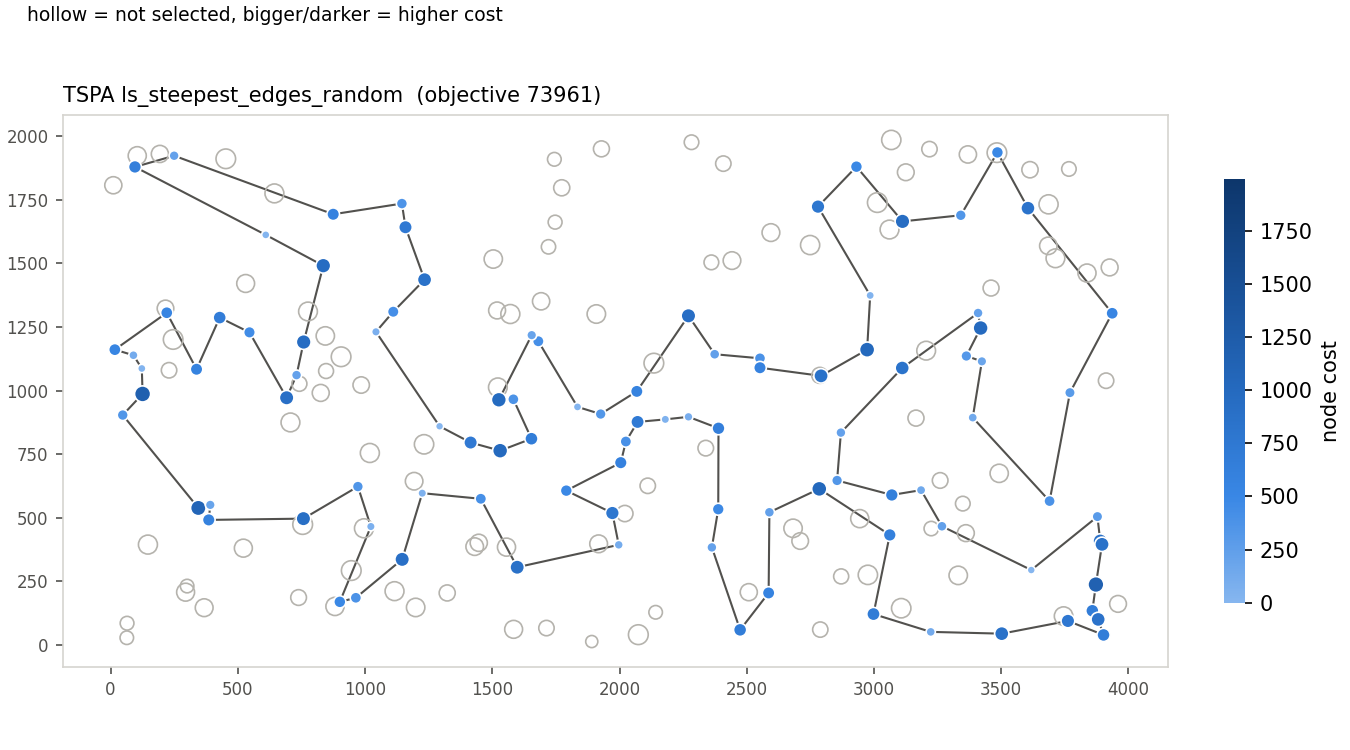
\includegraphics[width=0.85\textwidth]{plots/TSPA_ls_steepest_edges_random.png}
  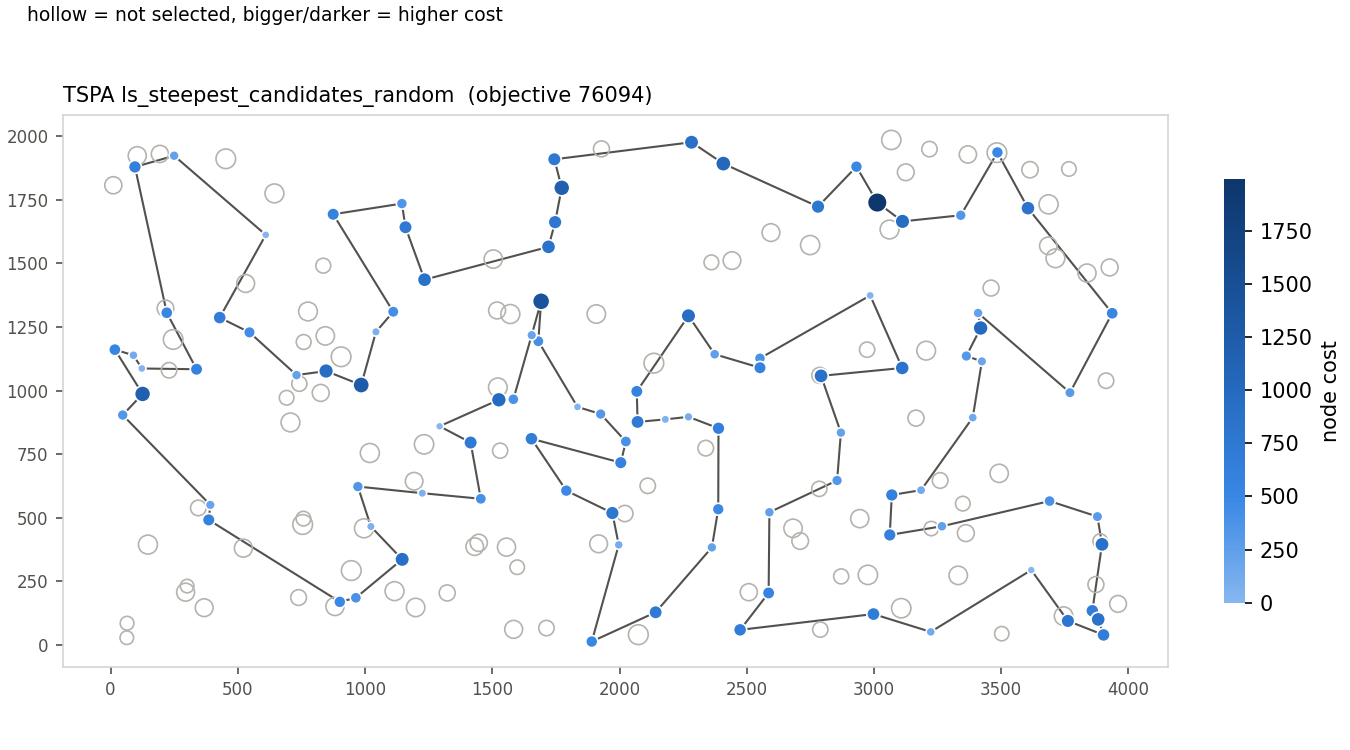
\includegraphics[width=0.85\textwidth]{plots/TSPA_ls_steepest_candidates_random.png}
\end{figure}
\begin{figure}[H]
  \centering
  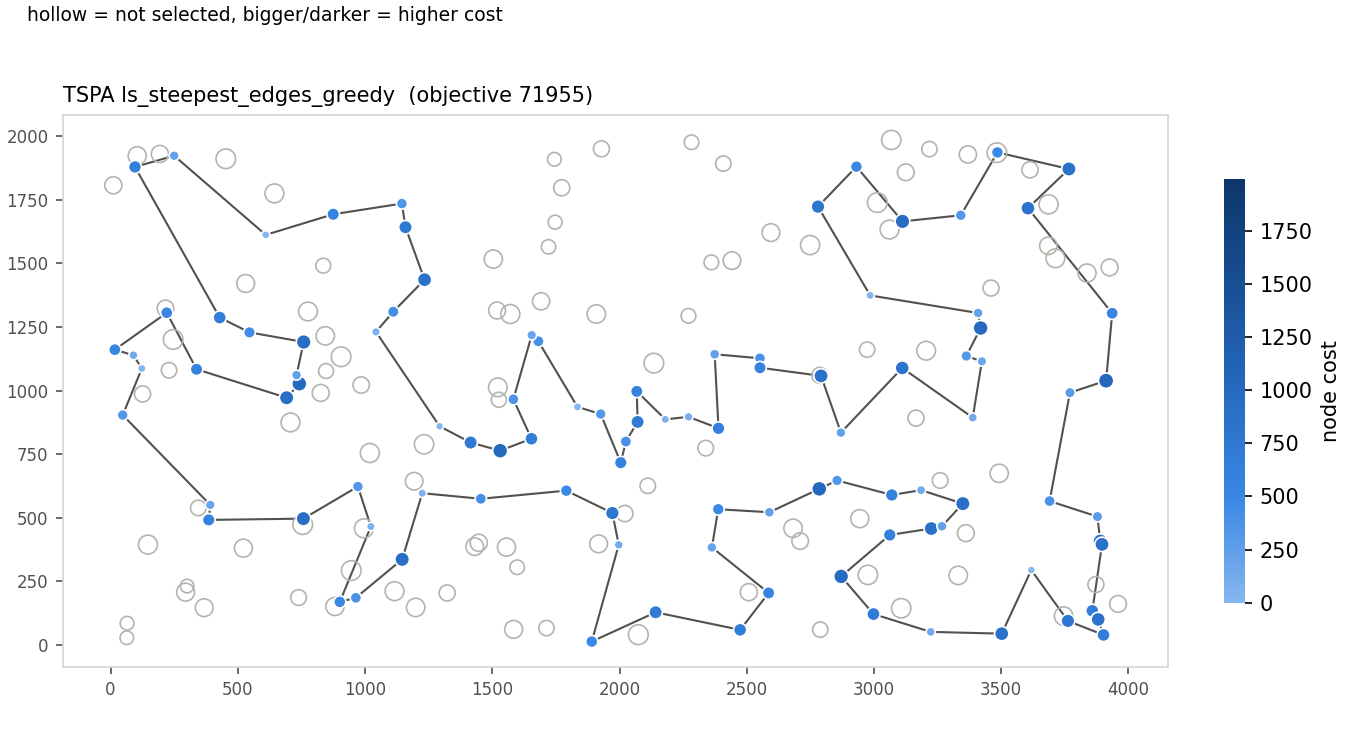
\includegraphics[width=0.85\textwidth]{plots/TSPA_ls_steepest_edges_greedy.png}
  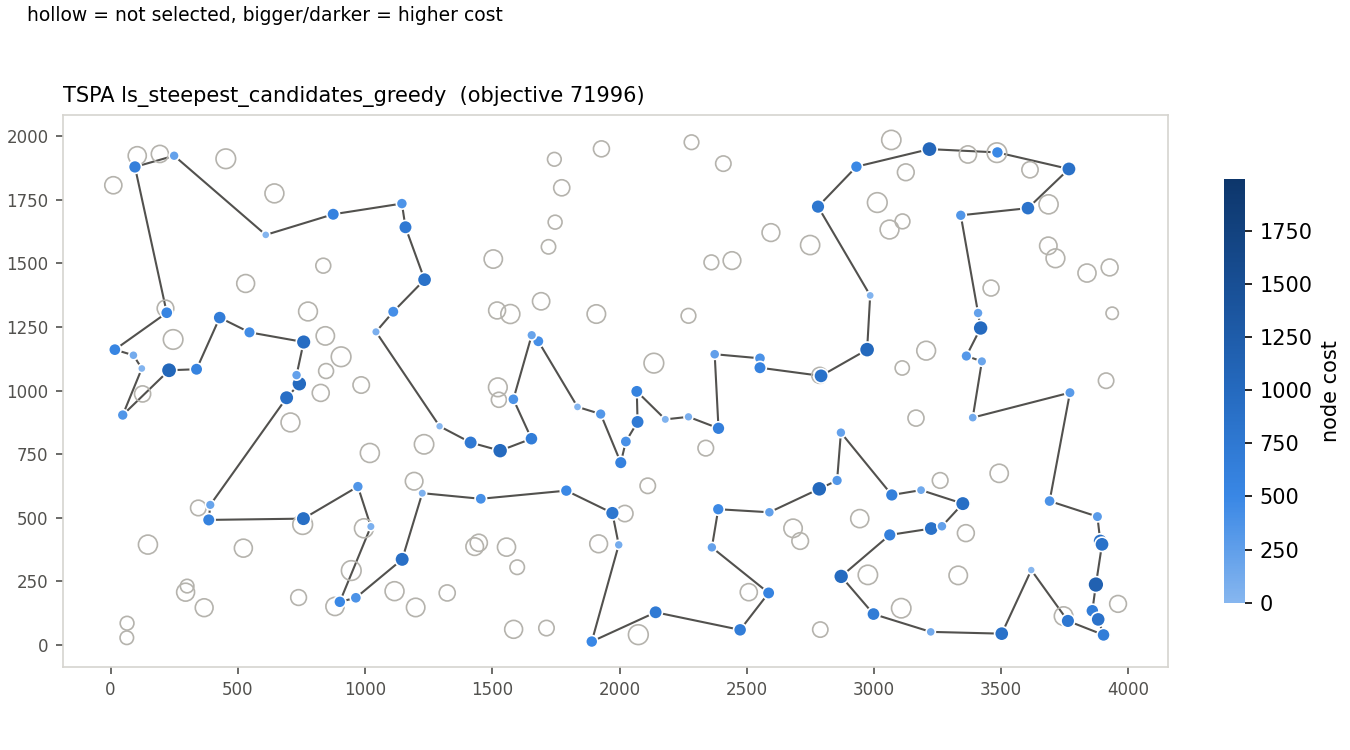
\includegraphics[width=0.85\textwidth]{plots/TSPA_ls_steepest_candidates_greedy.png}
\end{figure}
\subsection*{TSPB}
\begin{figure}[H]
  \centering
  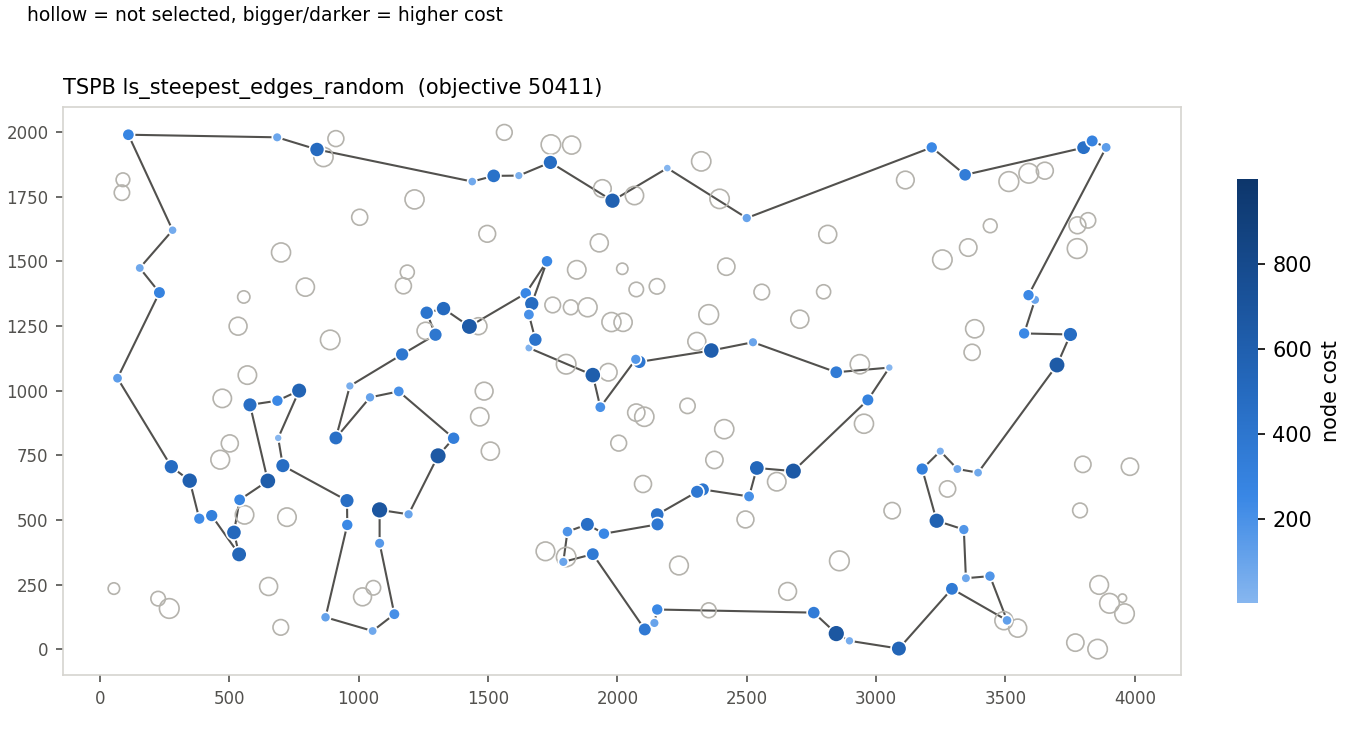
\includegraphics[width=0.85\textwidth]{plots/TSPB_ls_steepest_edges_random.png}
  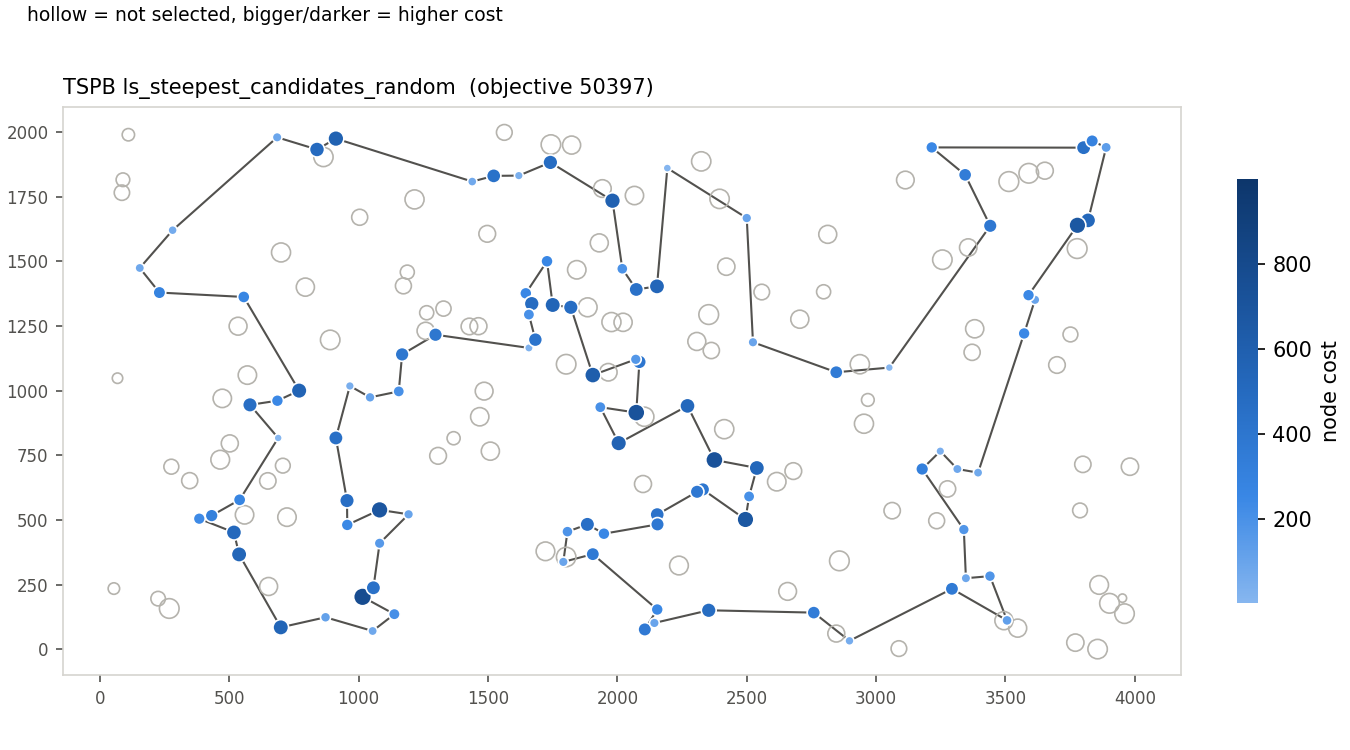
\includegraphics[width=0.85\textwidth]{plots/TSPB_ls_steepest_candidates_random.png}
\end{figure}
\begin{figure}[H]
  \centering
  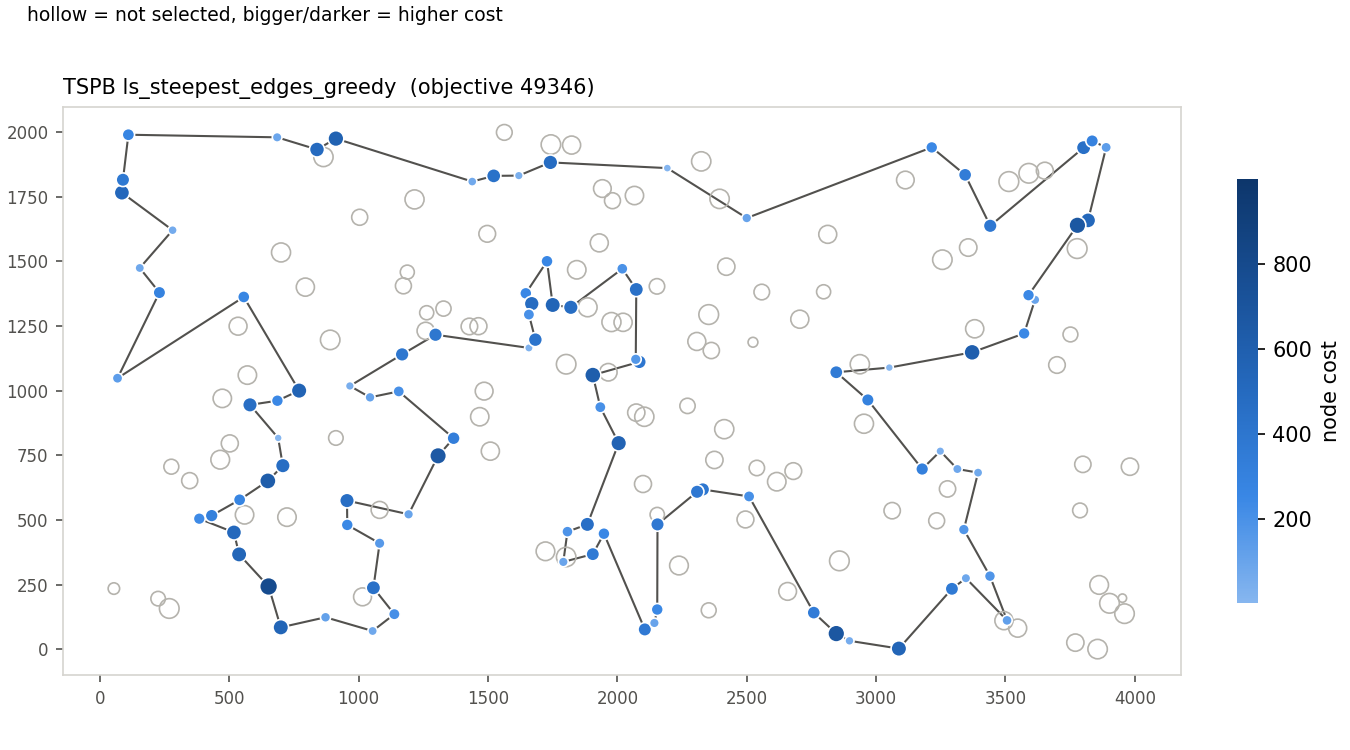
\includegraphics[width=0.85\textwidth]{plots/TSPB_ls_steepest_edges_greedy.png}
  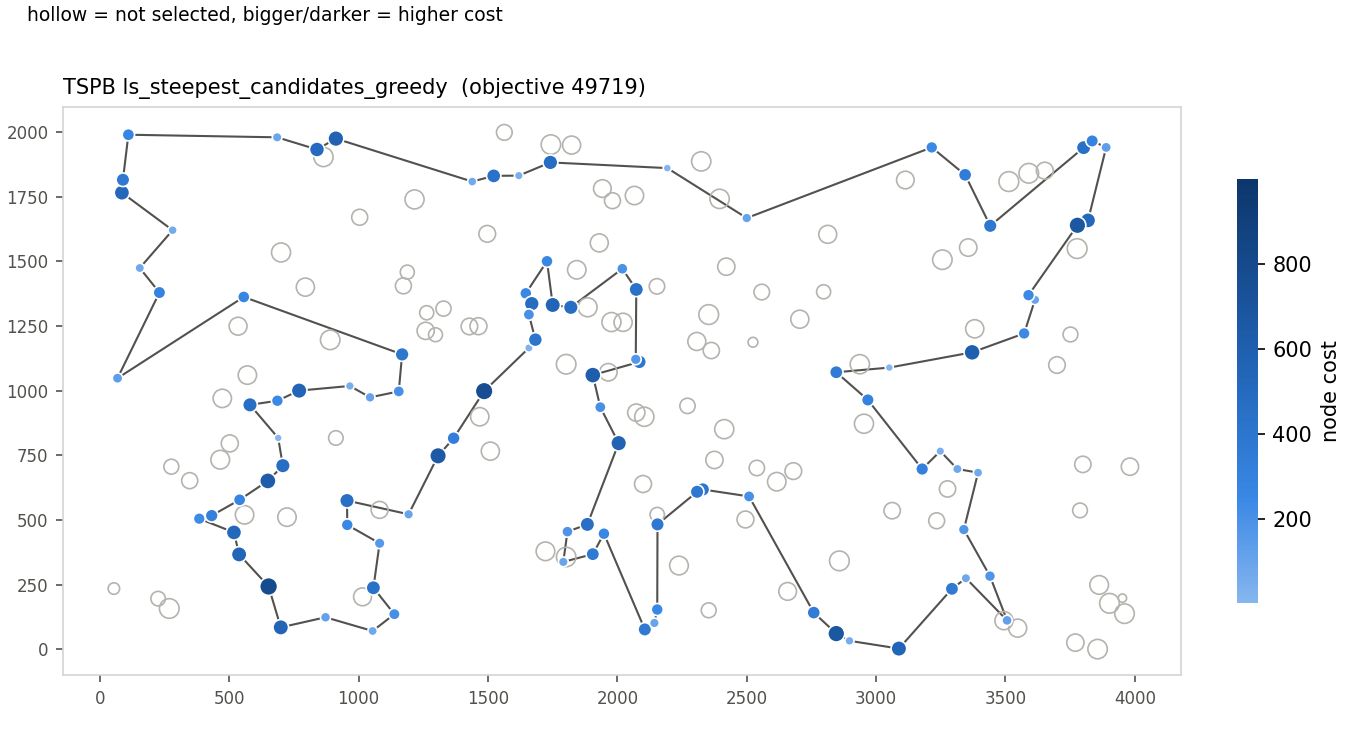
\includegraphics[width=0.85\textwidth]{plots/TSPB_ls_steepest_candidates_greedy.png}
\end{figure}

% ---------------------------------------------------------------
\section{Best solutions}
Lists of node indices, starting from 0, in the order they are visited. The cycle closes from the
last node back to the first. Best solutions of the previous methods are listed in the previous
reports.

\subsection*{TSPA}
\textbf{Baseline: LS steepest, two-edges, random start} (objective 73961)
\nodelist{127, 161, 30, 187, 171, 2, 189, 141, 87, 98, 135, 73, 45, 140, 53, 179, 177, 36, 131, 84, 58, 192, 158, 134, 72, 151, 182, 57, 64, 88, 78, 193, 153, 75, 170, 146, 159, 107, 89, 106, 150, 176, 174, 85, 1, 169, 3, 50, 93, 130, 47, 147, 101, 29, 178, 184, 136, 186, 164, 142, 8, 54, 9, 33, 143, 52, 144, 67, 16, 51, 156, 35, 185, 102, 28, 180, 132, 76, 4, 71, 157, 91, 48, 31, 80, 38, 100, 123, 160, 152, 108, 49, 60, 116, 149, 63, 119, 168, 95, 97}

\textbf{LS steepest, candidate moves, random start} (objective 76094)
\nodelist{176, 134, 158, 192, 182, 57, 107, 88, 78, 193, 153, 170, 159, 130, 89, 151, 150, 106, 93, 50, 3, 169, 1, 47, 147, 101, 29, 178, 184, 195, 136, 186, 154, 39, 115, 5, 112, 139, 4, 71, 157, 91, 76, 132, 162, 90, 123, 152, 108, 80, 48, 31, 60, 49, 63, 149, 116, 119, 168, 97, 127, 171, 2, 189, 187, 30, 141, 87, 28, 180, 156, 35, 51, 133, 16, 67, 144, 53, 140, 185, 45, 73, 135, 114, 181, 58, 84, 131, 36, 177, 179, 52, 143, 33, 54, 9, 164, 85, 8, 174}

\textbf{Baseline: LS steepest, two-edges, greedy start} (objective 71955)
\nodelist{101, 147, 37, 47, 130, 159, 146, 170, 153, 193, 78, 88, 107, 64, 57, 182, 138, 151, 42, 89, 113, 106, 150, 176, 72, 134, 84, 58, 158, 192, 181, 114, 135, 73, 45, 87, 141, 189, 2, 171, 187, 30, 161, 127, 97, 168, 63, 149, 116, 60, 49, 160, 83, 123, 100, 152, 108, 31, 48, 80, 91, 157, 71, 4, 76, 132, 180, 28, 102, 185, 35, 51, 16, 67, 144, 140, 53, 179, 52, 177, 36, 131, 33, 9, 54, 8, 174, 85, 93, 50, 3, 169, 1, 164, 186, 136, 184, 178, 29, 55}

\textbf{LS steepest, candidate moves, greedy start} (objective 71996)
\nodelist{60, 116, 149, 63, 168, 11, 49, 108, 152, 100, 123, 83, 160, 97, 127, 161, 30, 187, 171, 2, 189, 141, 87, 45, 73, 135, 114, 181, 192, 158, 58, 84, 134, 72, 176, 174, 150, 106, 113, 89, 42, 151, 138, 182, 57, 64, 107, 88, 78, 193, 153, 75, 170, 146, 159, 130, 47, 93, 50, 3, 169, 1, 178, 101, 55, 29, 163, 136, 186, 164, 142, 8, 54, 9, 33, 131, 36, 177, 52, 179, 53, 140, 144, 67, 16, 51, 35, 185, 102, 28, 180, 132, 76, 4, 71, 157, 91, 80, 48, 31}

\subsection*{TSPB}
\textbf{Baseline: LS steepest, two-edges, random start} (objective 50411)
\nodelist{197, 36, 29, 132, 103, 178, 65, 145, 28, 149, 37, 116, 147, 121, 198, 96, 48, 156, 89, 57, 190, 70, 81, 94, 105, 196, 114, 10, 148, 143, 90, 129, 127, 80, 182, 153, 20, 14, 2, 74, 17, 171, 39, 99, 179, 87, 82, 51, 85, 59, 73, 167, 181, 152, 34, 24, 67, 66, 84, 192, 54, 162, 76, 135, 3, 184, 151, 122, 69, 160, 172, 136, 120, 133, 189, 183, 30, 21, 38, 154, 97, 140, 47, 64, 33, 40, 141, 60, 45, 134, 175, 71, 155, 115, 170, 26, 125, 177, 180, 6}

\textbf{LS steepest, candidate moves, random start} (objective 50397)
\nodelist{73, 59, 85, 51, 179, 82, 87, 88, 99, 171, 74, 2, 14, 20, 153, 80, 127, 129, 90, 10, 114, 196, 139, 61, 105, 94, 81, 190, 70, 187, 54, 162, 76, 57, 89, 86, 46, 72, 156, 48, 96, 198, 121, 42, 147, 116, 149, 28, 145, 158, 26, 125, 177, 170, 6, 29, 132, 197, 36, 62, 175, 134, 45, 142, 157, 60, 40, 141, 71, 155, 97, 154, 140, 47, 38, 21, 69, 160, 172, 136, 133, 120, 8, 117, 122, 184, 3, 111, 151, 98, 27, 11, 66, 67, 31, 24, 34, 152, 181, 167}

\textbf{Baseline: LS steepest, two-edges, greedy start} (objective 49346)
\nodelist{65, 145, 28, 149, 13, 146, 37, 116, 147, 42, 121, 198, 96, 48, 89, 57, 190, 70, 187, 81, 94, 105, 61, 139, 196, 114, 10, 78, 54, 162, 192, 80, 127, 129, 90, 153, 14, 2, 20, 74, 17, 171, 39, 99, 67, 24, 34, 181, 179, 87, 82, 167, 51, 85, 59, 73, 98, 151, 122, 3, 184, 46, 72, 117, 8, 120, 133, 136, 172, 160, 69, 21, 38, 154, 140, 47, 64, 33, 40, 155, 71, 60, 157, 45, 134, 175, 62, 91, 36, 197, 132, 29, 6, 180, 115, 170, 177, 125, 26, 158}

\textbf{LS steepest, candidate moves, greedy start} (objective 49719)
\nodelist{65, 145, 28, 149, 13, 146, 37, 116, 147, 42, 121, 198, 96, 48, 89, 57, 190, 70, 187, 81, 94, 105, 61, 139, 196, 114, 10, 78, 54, 162, 192, 80, 127, 129, 90, 153, 14, 2, 20, 74, 17, 171, 39, 99, 67, 24, 34, 181, 179, 87, 82, 167, 51, 85, 59, 73, 98, 151, 122, 3, 184, 46, 72, 117, 8, 120, 133, 136, 172, 160, 69, 124, 64, 33, 40, 155, 71, 60, 157, 45, 134, 175, 62, 91, 36, 197, 132, 29, 6, 180, 115, 170, 177, 125, 26, 154, 140, 47, 38, 158}

% ---------------------------------------------------------------
\section{Solution checker}
All eight best solutions were checked with the provided solution checker
(\texttt{Solution checker.xlsx}), and every objective value matches. Our code additionally checks
every generated solution for the number of nodes and for repeated nodes.

Before the experiment we also tested the implementation: for 20 random solutions every generated
candidate move (39\,612 moves) was applied, and in all cases its delta was equal to the difference of
the full objective values, the move added at least one candidate edge, and $\mathit{pos}$ stayed
consistent with $P$. With $c = n - 1$ (every edge is a candidate edge) the result of the search had
no improving move in the full neighborhood of Lab~3.

\begin{table}[H]
\centering
\small
\begin{tabular}{llrrc}
\toprule
Instance & Method & Our objective & Checker objective & Match \\
\midrule
TSPA & Baseline (steepest, two-edges), random start & 73961 & 73961 & yes \\
TSPA & Steepest, candidate moves, random start & 76094 & 76094 & yes \\
TSPA & Baseline (steepest, two-edges), greedy start & 71955 & 71955 & yes \\
TSPA & Steepest, candidate moves, greedy start & 71996 & 71996 & yes \\
TSPB & Baseline (steepest, two-edges), random start & 50411 & 50411 & yes \\
TSPB & Steepest, candidate moves, random start & 50397 & 50397 & yes \\
TSPB & Baseline (steepest, two-edges), greedy start & 49346 & 49346 & yes \\
TSPB & Steepest, candidate moves, greedy start & 49719 & 49719 & yes \\
\bottomrule
\end{tabular}
\end{table}

% ---------------------------------------------------------------
\section{Conclusions}
\begin{itemize}
  \item From random starts, candidate moves make the steepest local search about 3.5 times faster:
        134.8\,ms instead of 464.6\,ms per run on TSPA and 129.1\,ms instead of 459.2\,ms on TSPB. The
        number of evaluated moves drops 8.5--8.7 times (about 230\,000 instead of 1\,990\,000 per run),
        because an iteration evaluates at most 2\,000 candidate moves instead of 14\,850. The time
        drops less than the number of moves, since generating the candidate moves (the loops over the
        lists and the look-ups in $\mathit{pos}$) also costs time.
  \item The number of iterations hardly changes (125--132 vs.\ 133), so the search makes about the
        same number of steps, each of them much cheaper.
  \item From greedy starts, candidate moves are also 3.8--4.6 times faster (4.5\,ms instead of
        21.1\,ms on TSPA, 18.6\,ms instead of 70.4\,ms on TSPB), and the quality is almost the same:
        the average is only 0.2\% worse on both instances (73\,181.4 vs.\ 73\,003.8 on TSPA,
        53\,196.9 vs.\ 53\,092.0 on TSPB). A greedy solution is already good, so only a few
        improving moves are left (2--15 iterations), and they are mostly local repairs that add
        short, cheap edges, so they are likely to be candidate moves. Even on TSPA, where candidate moves lose 5.3\% from random starts, the
        loss from greedy starts is small.
  \item The greedy start is much more important than the speed-up: the baseline from greedy starts
        is both better and faster than the candidate moves from random starts on TSPA (73\,003.8 in
        21.1\,ms vs.\ 80\,258.1 in 134.8\,ms). On TSPB the random starts still give the better average
        (52\,676.1 vs.\ 53\,092.0), as in Lab~3.
  \item On TSPB the quality is the same as without candidate moves (average 52\,676.1 vs.\
        52\,685.1), and the candidate version even found a slightly better best solution (50\,397 vs.\
        50\,411). Its average is the best of all methods so far on TSPB.
  \item On TSPA the quality is worse: the average grows by 5.3\% (80\,258.1 vs.\ 76\,184.6). The
        node costs of TSPA are twice as large as those of TSPB (up to 1\,997 vs.\ 999), so they
        dominate the score $D[u][v] + \mathit{cost}[v]$ and the 10 ``nearest'' nodes are often cheap
        but distant nodes, while short edges are left out. Indeed, 9 of the 100 edges of the best
        baseline solution of TSPA are not candidate edges for $c = 10$, compared with only 2 for
        TSPB. The search cannot add such edges, so it stops earlier in worse local optima.
  \item The number of candidate neighbors trades time for quality. The time grows roughly
        linearly with $c$ (about 62, 130, 197 and 264\,ms for $c = 5, 10, 15, 20$). With $c = 20$ the
        TSPA average (76\,621.4) is only 0.6\% above the baseline and the search is still 1.7 times
        faster; on TSPB already $c = 10$ is enough, and $c = 15$ or $20$ is slightly better than the
        baseline. Too few candidates ($c = 5$) clearly hurt on both instances.
\end{itemize}

\end{document}
